\part{統計学}

\chapter{統計学の目的}

まず,「統計学とは何のための学問か」についてまとめる.目的を理解した上で統計学の体系について説明する.

\section{統計学とは何のための学問か?}

\subsection{「データ」とは?}

統計学は「データの要約,解釈を行うための学問」であるが,そもそも「データ」とは何かを定義しておく.ざっくり言うと「データ = 事実,資料」である.

\begin{itemize}
  \item データ・・・立論・計算の基礎となる,既知のあるいは認容された事実,資料.
\end{itemize}

自然科学の分野では,しばしば「データ」,「事実」は,「現象(研究対象)を観測した際に得られる数値」,つまり「数値データ」を指すことが多い\footnote{数値データとしては個数,長さ,体積,重さ,特定の事柄が起こった回数,時刻,続いた時間の長さなどがある.}.

また,「データ」は数値データに限らず,文字,文書なども立派な「データ」である.数値データではないデータを統計学で扱う場合には,前処理として数値データへの変換などが行われた後に利用される.

\subsection{統計学とは?}

「統計学とはどのような学問か」という問いに対するいくつかの説明を挙げておく.

\begin{itemize}
  \item 数値データの要約,解釈を行う上での理論的根拠を提供するための学問
  \item (赤本\footnote{統計学入門(東京大学出版)}の説明を要約)数値データをどのように分析し,どのような判断を下したら良いかを論ずるための学問
  \item 対象とする集団,現象の数値データからその性質,法則性を導き出すための学問
\end{itemize}

\newpage

\section{統計学の体系:記述統計学と推測統計学}

「データに対する解釈を与える」という統計学の目的を達成するためにはどうすれば良いか?\\

ある現象の法則性を導くためには,まず,現象に関するデータを観測,取得する必要がある.
ここでは,「ある現象に関するデータを観測・取得済み」の状態を考える.
それらのデータから現象の法則性を導き出すためには,以下の 2 つの手順が考えられる.

\begin{itemize}
  \item データから現象の法則性を道きび出すための方法
        \begin{itemize}
          \item 手元のデータを丹念に調べ,その特徴,性質を調べ,現象の規則性,法則を見出す.
          \item 手元のデータを用い,「論理性のある」推測により現象の規則性,法則を見出す.
        \end{itemize}
\end{itemize}


上記手順はどちらも「統計学」が扱う範疇であるが,これらはそのまま統計学の分類に対応する.
前者は「\textbf{記述統計学}」\footnote{記述統計学,descriptive statistics},
後者は「\textbf{推測統計学}」\footnote{推測統計学,inferential statistics,inductive statistics}と呼ばれる学問に分類される.
ざっくり説明すると以下のようになる.

\begin{itemize}
  \item 統計学
        \begin{itemize}
          \item 記述統計学・・・手元のデータの説明
          \item 推測統計学・・・手元のデータから推測\footnote{正確には「手元のデータから『母集団の性質』の推測」}
        \end{itemize}
\end{itemize}

記述統計学と推測統計学の関係が非常に分かりやすく描かれているのが以下の図.後に出てくる統計学の用語が挙げられているが,ここでは雰囲気を掴む.

\begin{figure}[H]
  \begin{center}
    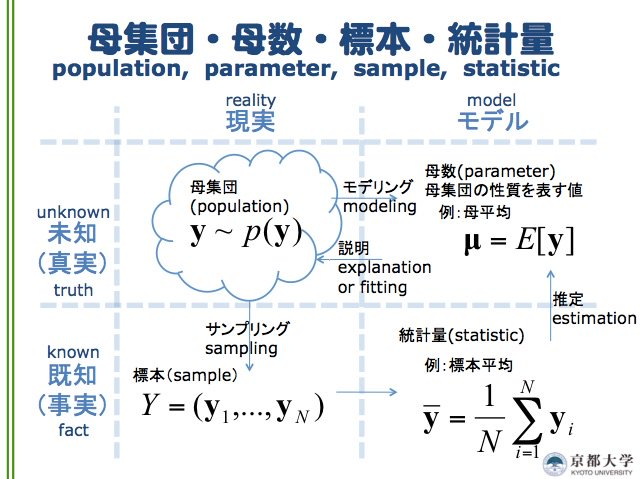
\includegraphics[width=15cm]{images/parts/1/statistics_map.jpeg}
    \caption{統計学の体系(hogeより引用)}
    % TODO: 引用元を探す
  \end{center}
\end{figure}

\section{記述統計学,推測統計学の基本的な流れ}

記述統計学,推測統計学の手法等を用いてデータ分析行う際の基本的な流れを説明する.

\subsection{データ分析における問題設定} % (fold)
\label{sub:データ分析における問題設定}

まず,データ分析の際に必ず行わなければならないのが「問題設定」である.
「〇〇という現象を理解したい」など,データ分析を行った結果何を得たいかという目的が必ず設定されているべきである.

また,\textbf{統計学はあくまでも「データに対する解釈を与える」ための手段の 1 つである},ということは認識しておくべきである.手段が目的となってはならない.
つまり,「統計学の〇〇という手法を使って△△という現象を理解したい」,「機械学習の△△という手法を使って何かできないか」ではなく,
「△△という現象を理解したい $\rightarrow$ その現象から得たデータに適した統計学(もしくは機械学習)の〇〇という手法を用いる」という順番であるべきである
\footnote{現実のデータ分析でこのような綺麗な流れがあるかは分からないが,少なくとも問題設定は必ず為されるべきである}.\\

まとめると,データ分析を行う際は,闇雲に統計学の手法を用いるのではなく,

\begin{enumerate}
  \item 「どんな現象を理解したいか」という\textbf{問題設定}
  \item 必要なデータの取得
  \item データの解釈,データから推測(必要であれば統計学の手法を用いる)
\end{enumerate}

という手順を踏むべきである.「問題設定 $\rightarrow$ データに適した統計学の手法の選択」という流れを意識したい.問題設定には例えば以下のようなものが考えられる.

\begin{itemize}
  \item 問題設定の例
        \begin{itemize}
          \item ある現象のデータからその傾向を見たい(記述統計学)
          \item 〇〇という仮説を検証したい(記述統計学,推測統計学)
          \item 手元のデータから未来のデータを予測したい(推測統計学)
        \end{itemize}
\end{itemize}

% subsection データ分析における問題設定 (end)

\newpage

\subsection{データ分析の流れ} % (fold)
\label{sub:データ分析の流れ}

前節を踏まえ,記述統計学,推測統計学の手法等を用いてデータ分析行う際の基本的な流れをざっくりまとめてみる.
両者の最終的なアウトプットの違いに着目すると良い.

\vspace{10pt}

\fbox{\parbox{\textwidth}{記述統計学の流れ
    \begin{enumerate}
      \item 問題設定,必要なデータを決める
      \item データの取得
      \item データの要約
      \item データの解釈
    \end{enumerate}
  }
}

\vspace{10pt}

\fbox{\parbox{\textwidth}{推測統計学の流れ
    \begin{enumerate}
      \item 問題設定,必要なデータを決める
      \item データの取得
      \item データから母集団の性質に当てはまる数理モデルを構築\footnote{統計モデル,時系列モデル,機械学習モデル,微分方程式モデルなど}
      \item 数理モデルを使った推定・推測・推論(データを生成する未知の真の確率分布)
      \item 数理モデルを使った推定・推測・推論の妥当性を考察・検証
    \end{enumerate}
  }
}
\vspace{10pt}

\begin{itemize}
  \item 記述統計学のアウトプット:対象となる現象,集団の性質,特徴の説明,解釈
  \item 推測統計学のアウトプット:対象となる現象,集団の性質,特徴の予測.例えば,「予測を行うための数理モデル」がアウトプットになる.この場合,「数理モデルの構築 $\rightarrow$ 検証」まで行って初めて意味を成す.
\end{itemize}


データ分析においては,上記の流れは上から下に綺麗に流れていくものではなく,上記の流れを回すである.
必要に応じて再度データ収集を行ったり,数理モデルの構築 $\rightarrow$ 検証のサイクルを回したり,といった

% subsectionデータ分析の流れ (end)

\section{補足 データの解釈:「定性的な解釈」と「定量的な解釈」}

統計学,または統計学だけでなくもっと広い意味で「データに対する解釈」を行う際に,解釈の結果として何らか(統計学で使われる指標など)の数値に落とし込むことが当たり前のように感じられるが,必ずしも数値に落とし込むことだけが「データに対する解釈」ではない\footnote{現実に統計学が使われる場面(データ分析など)では,アウトプットとして何らかの数値(指標)に落とし込むことが求められるのがほとんどだとは思いますが...}.
データに対する特徴・性質を「言葉」で表すこともできる.

\chapter{記述統計学} % (fold)
\label{cha:記述統計学}

% chapter 記述統計学 (end)

\chapter{推測統計学} % (fold)
\label{cha:推測統計学}

% chapter 推測統計学 (end)
